\section{Introduction}
Carbonic anhydrase (CA) catalyzes the interconversion of carbon dioxide and carbonic acid/bicarbonate as follows:
\begin{align}\label{eqn:ca_reaction}
\ce{CO_2 + H_2O 
<=>[\ce{CA}] 
H_2CO_3}
\end{align}
In the active form, CA is bound to a \ce{Zn^2+} cofactor (denoted as CA$\cdot$Zn), which it relies upon for its catalytic activity. The zinc ion can be stripped from the enzyme using a Lewis base ligand, which donates electrons to the ion to form a covalent bond. The ligand being studied in this experiment is 2,6-pyridinecarboxylate, commonly called dipicolinate (or dipic). Figure \ref{fig:dipic} shows the structure of dipic. In this experiment, the rate of zinc removal by dipic will be measured.
\begin{figure}[h]
  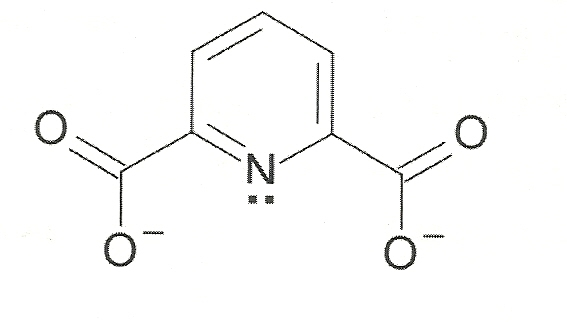
\includegraphics[scale=0.5]{./Figures/dipic.jpg}\\
  \caption{Structure of 2,6-pyridinecarboxylate (dipic)\cite{bib:lab_manual}}\label{fig:dipic}
\end{figure}
 
\subsection{Mechanism}
When $[dipic] >> [CA]$, that is, when $\frac{[dipic]}{[CA]} \ge 25$, then the removal of zinc is pseudo-first-order with respect to CA$\cdot$Zn because the concentration of dipic, denoted as L, does not change appreciably. Thus the formation of the inactive enzyme, apoCA, can be modeled using the following rate equation:
\begin{equation}\label{eqn:a}
\frac{d[\text{apoCA}]}{dt}=k_{obs}[\text{CA$\cdot$Zn}]
\end{equation}
The pseudo-first-order rate constant, $k_{obs}$, increases as [L] increases, but levels off at sufficiently high concentrations of L. Biochemists will recognize behavior similar to Michaelis-Menten enzyme kinetics in which the enzyme, CA$\cdot$Zn, and the substrate, L, reversibly form a CA$\cdot$Zn$\cdot$L complex with association constant $K_{EML}$ (EML stands for Enzyme-Metal-Ligand):
\begin{align}\label{eqn:KEML_reaction}
\ce{CA$\cdot$Zn + L
<=>[\ce{K_{EML}}]
CA$\cdot$Zn$\cdot$L}
\end{align}
This can be modeled as follows:
\begin{equation}\label{eqn:KEML_expression}
K_{EML}=\frac{\text{[CA$\cdot$Zn$\cdot$L]}}{\text{[CA$\cdot$Zn][L]}}
\end{equation}

CA$\cdot$Zn$\cdot$L can either revert back to the original species or irreversibly convert to the inactive form of the enzyme, apoCA, and the covalently bound zinc-dipic molecule, ZnL:
\begin{align}\label{eqn:kd_reaction}
\ce{CA$\cdot$Zn$\cdot$L
->[\ce{k_{d}}]
apoCA + ZnL}
\end{align}
This yields the following differential rate law:
\begin{equation}\label{eqn:kd_expression}
\frac{d[\text{apoCA}]}{dt}=k_{d}[\text{CA$\cdot$Zn$\cdot$L}]
\end{equation}

Recall that $\text{[L]} >> \text{[CA$\cdot$Zn]}$, so $[L]$ can be assumed to stay constant at $\text{[L]}_0$